%%%%%%%%%%%%%%%%%%%%%%%%%%%%%%%%%%%%%%%%%%%%%%%%%%%%%%%%%%%%%%%%%%%%%%%%%%%%%%%%
%2345678901234567890123456789012345678901234567890123456789012345678901234567890
%        1         2         3         4         5         6         7         8

%\documentclass[letterpaper, 10 pt, conference]{ieeeconf}  % Comment this line out
                                                          % if you need a4paper
\documentclass[a4paper, 10pt, conference]{ieeeconf}      % Use this line for a4
                                                          % paper

\pagestyle{plain}

\IEEEoverridecommandlockouts                              % This command is only
                                                          % needed if you want to
                                                          % use the \thanks command
\overrideIEEEmargins
% See the \addtolength command later in the file to balance the column lengths
% on the last page of the document

\usepackage[utf8]{inputenc}
\usepackage[T1]{fontenc}

\usepackage{cite}
%\usepackage{amsmath,amssymb,amsfonts}
\usepackage{algorithmic}
\usepackage{graphicx}
\usepackage{textcomp}
\usepackage{xcolor}



% The following packages can be found on http:\\www.ctan.org
\usepackage{epsfig} % for postscript graphics files
\usepackage{mathptmx} % assumes new font selection scheme installed
\usepackage{mathptmx} % assumes new font selection scheme installed
\usepackage{amsmath} % assumes amsmath package installed
\usepackage{amssymb}  % assumes amsmath package installed

\def\BibTeX{{\rm B\kern-.05em{\sc i\kern-.025em b}\kern-.08em
    T\kern-.1667em\lower.7ex\hbox{E}\kern-.125emX}}

\title{\LARGE \bf
Title of Mechatronics and Power Electronics Project Report
}

%\author{ \parbox{3 in}{\centering Huibert Kwakernaak*
%         \thanks{*Use the $\backslash$thanks command to put information here}\\
%         Faculty of Electrical Engineering, Mathematics and Computer Science\\
%         University of Twente\\
%         7500 AE Enschede, The Netherlands\\
%         {\tt\small h.kwakernaak@autsubmit.com}}
%         \hspace*{ 0.5 in}
%         \parbox{3 in}{ \centering Pradeep Misra**
%         \thanks{**The footnote marks may be inserted manually}\\
%        Department of Electrical Engineering \\
%         Wright State University\\
%         Dayton, OH 45435, USA\\
%         {\tt\small pmisra@cs.wright.edu}}
%}

\author{Student LastName, StudentSecond Last2Name, and Supervisor LastSupName% <-this % stops a space
%\thanks{*This work was not supported by any organization}% <-this % stops a space
\thanks{ S. LastName, S. Last2Name, and Supervisor LastSupName are with Mechatronics and Power Electronics Institute (MPEI),
        TU Wien, 1040 Vienna, Austria
        {\tt\small studentemail at tuwien.ac.at}}%
}

\begin{document}



\maketitle
%\thispagestyle{empty}
%\pagestyle{empty}
\thispagestyle{plain}
\pagestyle{plain}


%%%%%%%%%%%%%%%%%%%%%%%%%%%%%%%%%%%%%%%%%%%%%%%%%%%%%%%%%%%%%%%%%%%%%%%%%%%%%%%%
\begin{abstract}

This document is a model and instructions for the final report of Mechatronics and Power Electronics (MPE) project using \LaTeX.
This and the style file, IEEEtran.cls, define the components of your paper [title, text, heads, etc.]. *CRITICAL: Do Not Use Symbols, Special Characters, Footnotes, 
or Math in Paper Title or Abstract. 

\end{abstract}

\begin{keywords}
add five keywords, formatting, style, styling, insert
\end{keywords}

%%%%%%%%%%%%%%%%%%%%%%%%%%%%%%%%%%%%%%%%%%%%%%%%%%%%%%%%%%%%%%%%%%%%%%%%%%%%%%%%
\section{Introduction}

This template provides authors with most of the formatting specifications needed for preparing electronic versions of their papers. The IEEE conference paper template is taken as a basis while there are some minor rules of writing need to considered, which was discussed in the lecture ``How to conduct research and write a report''. Please check the material so that your report is well structured and presented your achievements in the project. The total page number should be from 6 to 8 pages for a brief description of your project. If there is additional information you want to write, please provide them a separated appendix document. There is no format and limitation in page number for this appendix. 


\section{Basics}
All standard paper components have been specified for three reasons: (1) ease of use when formatting individual papers, (2) automatic compliance to electronic requirements that facilitate the concurrent or later production of electronic products, and (3) conformity of style throughout reports. Margins, column widths, line spacing, and type styles are built-in; examples of the type styles are provided throughout this document and are identified in italic type, within parentheses, following the example. The student may need to create necessary components, incorporating the applicable criteria that follow.

\subsection{Page Setting}

First, confirm that you have the correct template for your paper size. This template has been tailored for output on the A4 paper. Please do not use it for US-letter paper size since the margin requirements for A4 papers may be different from A4 paper.

\subsection{Filename of the Final Report}

The file name is set to the initial of the author, course initial of ``MPE'', academic year, semester (WS- winter semester and SS- summer semester), and short title of project without space. For example, the first author is Student LastName, then ``SL\_MPE2022WS\_ProjectShortTitle.tex'' to generate ``SL\_MPE2022WS\_ProjectShortTitle.pdf'

\subsection{Languages}

You can use either German or English. Discuss it in advance with your supervisor. 

\subsection{Submission with the Final Report}

With the final report, students are asked to submit all files related to the projects, e.g. or any related documents and files for design, simulation, materials, datasheet of used systems, and so on. This will help us to achieve your work for further development of the project and will also help new students who want to continue your project. Please achieve it as a zip file and give it to the supervisor so that he can upload the results in the MPEI network drive. 

\subsection{Maintaining the Integrity of the Specifications}

The template is used to format your paper and style the text. All margins, column widths, line spaces, and text fonts are prescribed; please do not alter them. You may note peculiarities. For example, the head margin in this template measures proportionately more than is customary. This measurement and others are deliberate, using specifications that anticipate your paper as one part of the entire proceedings, and not as an independent document. Please do not revise any of the current designations

\section{Prepare Your Paper before Styling}

Before you begin to format your paper, first write and save the content as a separate text file. Keep your text and graphic files separate until after the text has been formatted and styled. Do not use hard tabs, and limit use of hard returns to only one return at the end of a paragraph. 

Finally, complete content and organizational editing before formatting. Please take note of the following items when proofreading spelling and grammar:

\subsection{Abbreviations and Acronyms} Define abbreviations and acronyms the first time they are used in the text, even after they have been defined in the abstract. Abbreviations such as IEEE, SI, MKS, CGS, sc, dc, and rms do not have to be defined. Do not use abbreviations in the title or heads unless they are unavoidable.

\subsection{Units}

\begin{itemize}

\item Use either SI (MKS) or CGS as primary units. (SI units are encouraged.) English units may be used as secondary units (in parentheses). An exception would be the use of English units as identifiers in trade, such as ``3.5-inch disk drive''.
\item Avoid combining SI and CGS units, such as current in amperes and magnetic field in oersteds. This often leads to confusion because equations do not balance dimensionally. If you must use mixed units, clearly state the units for each quantity that you use in an equation.
\item Do not mix complete spellings and abbreviations of units: ``Wb/m2'' or ``webers per square meter'', not ``webers/m2''.  Spell out units when they appear in text: ``\ldots a few henries'', not ``\ldots a few H''.
\item Use a zero before decimal points: ``0.25'', not ``.25''. Use ``cm$^3$'', not ``cc''. (bullet list)

\end{itemize}


\subsection{Equations}

The equations are an exception to the prescribed specifications of this template. You will need to determine whether or not your equation should be typed using either the Times New Roman or the Symbol font (please no other font). To create multileveled equations, it may be necessary to treat the equation as a graphic and insert it into the text after your paper is styled. Number equations consecutively. Equation numbers, within parentheses, are to position flush right, as in (1), using a right tab stop. To make your equations more compact, you may use the solidus ( / ), the exp function, or appropriate exponents. Italicize Roman symbols for quantities and variables, but not Greek symbols. Use a long dash rather than a hyphen for a minus sign. Punctuate equations with commas or periods when they are part of a sentence, as in
\begin{equation}
\alpha + \beta = \chi, \label{Eq:addition}
\end{equation}
where $\alpha$ denotes \ldots. Define 
\begin{align}
\zeta &= \alpha - \beta  \nonumber \\ 
			&= \chi - 2\beta.  \label{Eq:substraction}
\end{align}

Note that the equation is centered using a center tab stop. Be sure that the symbols in your equation have been defined before or immediately following the equation. Use ``(\ref{Eq:addition})'', not ``Eq.~(\ref{Eq:addition})'' or ``equation (\ref{Eq:addition})'', except at the beginning of a sentence: ``Equation (\ref{Eq:substraction}) is\ldots''


\subsection{\LaTeX-Specific Advice}

Please use ``soft'' (e.g., \verb|\eqref{Eq}|) cross references instead
of ``hard'' references (e.g., \verb|(1)|). That will make it possible
to combine sections, add equations, or change the order of figures or
citations without having to go through the file line by line.

Please don't use the \verb|{eqnarray}| equation environment. Use
\verb|{align}| or \verb|{IEEEeqnarray}| instead. The \verb|{eqnarray}|
environment leaves unsightly spaces around relation symbols.

Please note that the \verb|{subequations}| environment in {\LaTeX}
will increment the main equation counter even when there are no
equation numbers displayed. If you forget that, you might write an
article in which the equation numbers skip from (17) to (20), causing
the copy editors to wonder if you've discovered a new method of
counting.

{\BibTeX} does not work by magic. It doesn't get the bibliographic
data from thin air but from .bib files. If you use {\BibTeX} to produce a
bibliography you must send the .bib files. 

{\LaTeX} can't read your mind. If you assign the same label to a
subsubsection and a table, you might find that Table I has been cross
referenced as Table IV-B3. 

{\LaTeX} does not have precognitive abilities. If you put a
\verb|\label| command before the command that updates the counter it's
supposed to be using, the label will pick up the last counter to be
cross referenced instead. In particular, a \verb|\label| command
should not go before the caption of a figure or a table.

Do not use \verb|\nonumber| inside the \verb|{array}| environment. It
will not stop equation numbers inside \verb|{array}| (there won't be
any anyway) and it might stop a wanted equation number in the
surrounding equation.


\subsection{Some Common Mistakes}
\begin{itemize}


\item The word ``data'' is plural, not singular.
\item The subscript for the permeability of vacuum ?0, and other common scientific constants, is zero with subscript formatting, not a lowercase letter ``o''.
\item In American English, commas, semi-/colons, periods, question and exclamation marks are located within quotation marks only when a complete thought or name is cited, such as a title or full quotation. When quotation marks are used, instead of a bold or italic typeface, to highlight a word or phrase, punctuation should appear outside of the quotation marks. A parenthetical phrase or statement at the end of a sentence is punctuated outside of the closing parenthesis (like this). (A parenthetical sentence is punctuated within the parentheses.)
\item A graph within a graph is an ``inset'', not an ``insert''. The word alternatively is preferred to the word ``alternately'' (unless you really mean something that alternates).
\item Do not use the word ``essentially'' to mean ``approximately'' or ``effectively''.
\item In your paper title, if the words ``that uses'' can accurately replace the word ``using'', capitalize the ``u''; if not, keep using lower-cased.
\item Be aware of the different meanings of the homophones ``affect'' and ``effect'', ``complement'' and ``compliment'', ``discreet'' and ``discrete'', ``principal'' and ``principle''.
\item Do not confuse ``imply'' and ``infer''.
\item The prefix ``non'' is not a word; it should be joined to the word it modifies, usually without a hyphen.
\item There is no period after the ``et'' in the Latin abbreviation ``et al.''.
\item The abbreviation ``i.e.'' means ``that is'', and the abbreviation ``e.g.'' means ``for example''.

\end{itemize}

\section{Further Use of the Template}

Use this sample document as your LaTeX source file to create your document. Save this file , for example, as root.tex. You have to make sure to use the cls file that came with this distribution. If you use a different style file, you cannot expect to get required margins. Note also that when you are creating your out PDF file, the source file is only part of the equation.

\subsection{Headings, etc}

Text heads organize the topics on a relational, hierarchical basis. For example, the paper title is the primary text head because all subsequent material relates and elaborates on this one topic. If there are two or more sub-topics, the next level head (uppercase Roman numerals) should be used and, conversely, if there are not at least two sub-topics, then no subheads should be introduced. Styles named ``Heading 1'', ``Heading 2'', ``Heading 3'', and ``Heading 4'' are prescribed.

\subsection{Figures and Tables}

Positioning Figures and Tables: Place figures and tables at the top and bottom of columns. Avoid placing them in the middle of columns. Large figures and tables may span across both columns. Figure captions should be below the figures; table heads should appear above the tables. Insert figures and tables after they are cited in the text. Use the abbreviation ``Fig.~\ref{fig:AFMResponse}'', even at the beginning of a sentence.

\begin{figure}[t]% [tbph]
\centerline{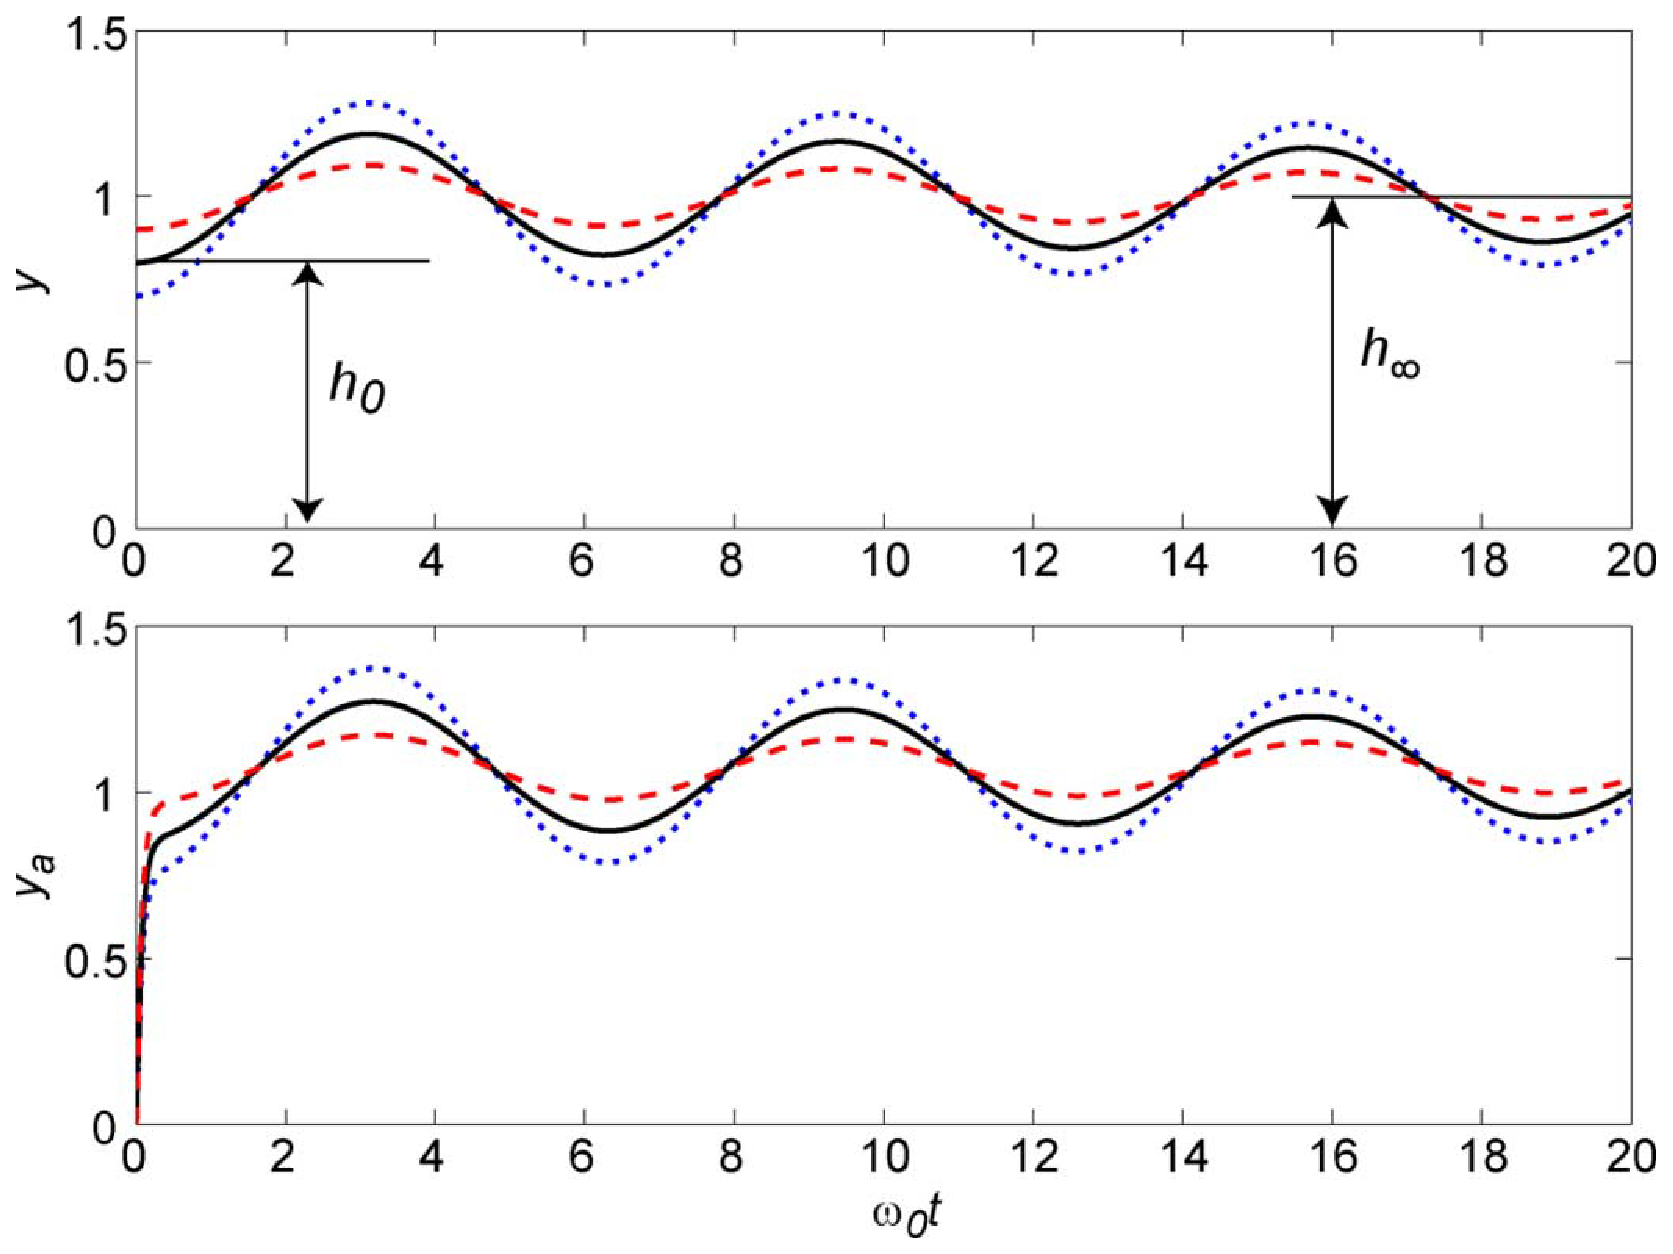
\includegraphics[width=0.49\textwidth]{testImg.eps}}
\caption{Upper curves: Simulated step response of the scanner in Z-direction for $\zeta = 0.02$ and $\alpha = 0.7$ (dotted blue line), $0.8$ (solid black line) and $0.9$ (dashed
red line). The lower curves show the step response when a time constant of the piezo amplifier of $\tau = 0:07/\omega_0$ is added \cite{schitterDesignModelingHighSpeed2007}. For images, If possible, try to use {\bf vector images (eps files)} as much as possible with embedded fonts.}
\label{fig:AFMResponse}
\end{figure}

\begin{table}[t]%[tbph]
\caption{Table Type Styles}
\begin{center}
\begin{tabular}{|c|c|c|c|}
\hline
\textbf{Table}&\multicolumn{3}{|c|}{\textbf{Table Column Head}} \\
\cline{2-4} 
\textbf{Head} & \textbf{\textit{Table column subhead}}& \textbf{\textit{Subhead}}& \textbf{\textit{Subhead}} \\
\hline
copy& More table copy$^{\mathrm{a}}$& &  \\
\hline
\multicolumn{4}{l}{$^{\mathrm{a}}$Sample of a Table footnote.}
\end{tabular}
\label{Table:ex1}
\end{center}
\end{table}


   %\begin{figure}[thpb]
      %\centering
      %\framebox{\parbox{3in}{We suggest that you use a text box to insert a graphic (which is ideally a 300 dpi TIFF or EPS file, with all fonts embedded) because, in an document, this method is somewhat more stable than directly inserting a picture.
%}}
      %%\includegraphics[scale=1.0]{figurefile}
      %\caption{Inductance of oscillation winding on amorphous
       %magnetic core versus DC bias magnetic field}
      %\label{figurelabel}
   %\end{figure}
   

Figure Labels: Use 8 point Times New Roman for Figure labels, which is managed in the style file of latex. Use words rather than symbols or abbreviations when writing Figure axis labels to avoid confusing the reader. As an example, write the quantity ``Magnetization'', or ``Magnetization, M'', not just ``M''. If including units in the label, present them within parentheses. Do not label axes only with units. In the example, write ``Magnetization (A/m)'' or ``Magnetization {A[m(1)]}'', not just ``A/m''. Do not label axes with a ratio of quantities and units. For example, write ``Temperature (K)'', not ``Temperature/K.''

\subsection{References}

Please number citations consecutively within brackets \cite{schitterDesignModelingHighSpeed2007}. The 
sentence punctuation follows the bracket \cite{oppenheimSignalsSystems2nd1996}. Refer simply to the reference 
number, as in \cite{MunnigSchmidtMechatronics2nd2014}---do not use ``Ref. \cite{MunnigSchmidtMechatronics2nd2014}'' or ``reference \cite{MunnigSchmidtMechatronics2nd2014}'' except at 
the beginning of a sentence: ``Reference \cite{MunnigSchmidtMechatronics2nd2014} was the first $\ldots$''

Number footnotes separately in superscripts. Place the actual footnote at 
the bottom of the column in which it was cited. Do not put footnotes in the 
abstract or reference list. Use letters for table footnotes.

 Papers that have not been published, even if they have been 
submitted for publication, should be cited as ``unpublished'' \cite{biagettiDiscreteBesselFunctions2016}. Papers 
that have been accepted for publication should be cited as ``in press'' \cite{VW8000Std}. 
Capitalize only the first word in a paper title, except for proper nouns and 
element symbols.  The multiple reference should be merged together, i.e. \cite{schitterDesignModelingHighSpeed2007,oppenheimSignalsSystems2nd1996,MunnigSchmidtMechatronics2nd2014}.
For papers published in translation journals, please give the English 
citation first, followed by the original foreign-language citation.


\section{Conclusion}

A conclusion section is required in the report. Although a conclusion may review the main points of the paper, do not replicate the abstract as the conclusion. A conclusion might elaborate on the importance of the work or suggest applications and extensions. 

\addtolength{\textheight}{-12cm}   % This command serves to balance the column lengths
                                  % on the last page of the document manually. It shortens
                                  % the textheight of the last page by a suitable amount.
                                  % This command does not take effect until the next page
                                  % so it should come on the page before the last. Make
                                  % sure that you do not shorten the textheight too much.

%%%%%%%%%%%%%%%%%%%%%%%%%%%%%%%%%%%%%%%%%%%%%%%%%%%%%%%%%%%%%%%%%%%%%%%%%%%%%%%%



%%%%%%%%%%%%%%%%%%%%%%%%%%%%%%%%%%%%%%%%%%%%%%%%%%%%%%%%%%%%%%%%%%%%%%%%%%%%%%%%



%%%%%%%%%%%%%%%%%%%%%%%%%%%%%%%%%%%%%%%%%%%%%%%%%%%%%%%%%%%%%%%%%%%%%%%%%%%%%%%%
\section*{Appendix}

If Appdendix is required, please do not add appendix in this report but provide it as a separated document. 

%\section*{Acknowledgment}
%
%If there is anyone who need to be acknowledged, write down here


%%%%%%%%%%%%%%%%%%%%%%%%%%%%%%%%%%%%%%%%%%%%%%%%%%%%%%%%%%%%%%%%%%%%%%%%%%%%%%%%
%References are important to the reader; therefore, each citation must be complete and correct. If at all possible, references should be commonly available publications.

\bibliographystyle{./IEEEtran}
\bibliography{./myBibliography}



\end{document}
